\documentclass[12pt]{article}
\usepackage{amsfonts}
\usepackage{amsmath}
\usepackage{graphicx}
\usepackage{xcolor}
\newcommand{\blue}[1]{\textcolor{blue}{#1}}
\usepackage{float}
\usepackage[caption = false]{subfig}
\usepackage{/Users/timbarry/optionFiles/mymacros}

\begin{document}
\noindent
Tim, Gene, Kathryn
\begin{center}
\textbf{A new class of measurement error models, with application to CRISPR genome editing and single-cell sequencing}
\end{center}

\section{Introduction}
CRISPR is a genome engineering tool that has enabled scientists to precisely edit human and nonhuman genomes, opening the door to new medical therapies \cite{Rothgangl2021,Musunuru2021} and transforming basic biology research \cite{Przybyla2021}. Recently, scientists have paired CRISPR genome engineering with single-cell sequencing \cite{Dixit2016,Datlinger2017}. The resulting assays, known as a ``single-cell CRISPR screens,'' link genetic perturbations in individual cells to changes in gene expression, illuminating regulatory networks underlying human diseases and other traits \cite{Morris2021a}.

Despite their promise, single-cell CRISPR screens present substantial statistical challenges. A major difficulty is that CRISPR perturbations are unobservable and assigned stochastically to cells. As a consequence, we cannot know with certainty which cells were perturbed. Instead, we must leverage an indirect, noisy proxy of perturbation presence or absence -- namely, transcribed barcode counts -- to ``guess'' which cells were perturbed. Using these imputed perturbation assignments, we can attempt to estimate the effect of the perturbation on gene expression. The standard approach, which we call the ``thresholding method,'' is to assign perturbation identities to cells by simply thresholding the barcode counts.

We study estimation and inference in single-cell CRISPR screens from a statistical perspective, formulating the data generating mechanism using a new class of errors-in-variables (or measurement error) models. We assume that the response variable $y$ is a GLM of an underlying predictor variable $x^*$. We do not observe $x^*$ directly; rather, we observe a noisy version $x$ of $x^*$ that itself is a GLM of $x^*$. The goal of the analysis is to estimate the effect of $x^*$ on $y$ using the observed data $(x , y)$ only. In the context of the biological application, $x^*$, $y$, and $x$ are CRISPR perturbations, gene expressions, and barcode counts, respectively.

Our work makes two main contributions. First, we study the thresholding method from empirical and theoretical perspectives. Notably, we demonstrate on real data that the thresholding method exhibits a bias-variance tradeoff as a function of the selected threshold, and we recover this phenomenon in precise mathematical terms in an idealized Gaussian model. Second, we introduce a new method for estimation and inference in single-cell CRISPR screens that accounts for the measurement error inherent in the experiment. The method, called \textit{GLM-EIV} (generalized linear model with errors-in-variables), implicitly estimates the probability that each cell was perturbed, obviating the need to explicitly impute perturbation assignments via thresholding or another heuristic. Theoretical analyses and simulation studies indicate that GLM-EIV outperforms the thresholding method in large regions of the parameter space.

We implement several statistical accelerations to bring the cost of GLM-EIV down to within an order of magnitude of the thresholding method. Finally, we develop a computational infrastructure to deploy GLM-EIV at-scale across hundreds or thousands of processors on clouds (e.g., Microsoft Azure) and high-performance clusters. Leveraging this infrastructure, we apply GLM-EIV to analyze two recent, large-scale, high multiplicity-of-infection single-cell CRISPR screen datasets, yielding new biological and statistical insights. 

\section{Background and analysis challenges}

Our focus in this work is on high multiplicity-of-infection (MOI), enhancer-targeting, single-cell CRISPR screens. In this section we cover relevant biological background and motivation.
\\ \\
\textbf{P1}: The human genome consists of genes (segments of DNA that code for proteins), enhancers (segments of DNA that regulate the expression of one or more genes), and other genomic regions. Genome-wide association studies have revealed that the majority ($>95\%$) of variants associated with diseases lie outside genes and (very likely) inside enhancers. These noncoding variants contribute to disease by modulating the expression one or more genes, which in turn encode proteins that affect the phenotype. A central open challenge in genetics, therefore, is to link enhancers that harbor disease-associated variants to the genes that they target at genome-wide scale.
\\ \\
\textbf{P2}: High MOI single-cell CRISPR screens are the most promising biotechnology for solving this problem. \blue{Describe the experimental protocol here. Explain that we use the terms ``barcodes'' and ``gRNAs'' interchangeably, as polyadenylated gRNAs serve as barcodes in CROP-seq. Link to Figure \ref{analysis_challenges}.}
\\ \\
\textbf{P3}: Single-cell CRISPR screens pose several core analysis challenges. \blue{Describe the analysis challenges here: (i) unobserved perturbation; (ii) existence of background reads; (iii) highly discrete count data; (iv) nuisance variables}.

\begin{figure}[h!]
	\centering
	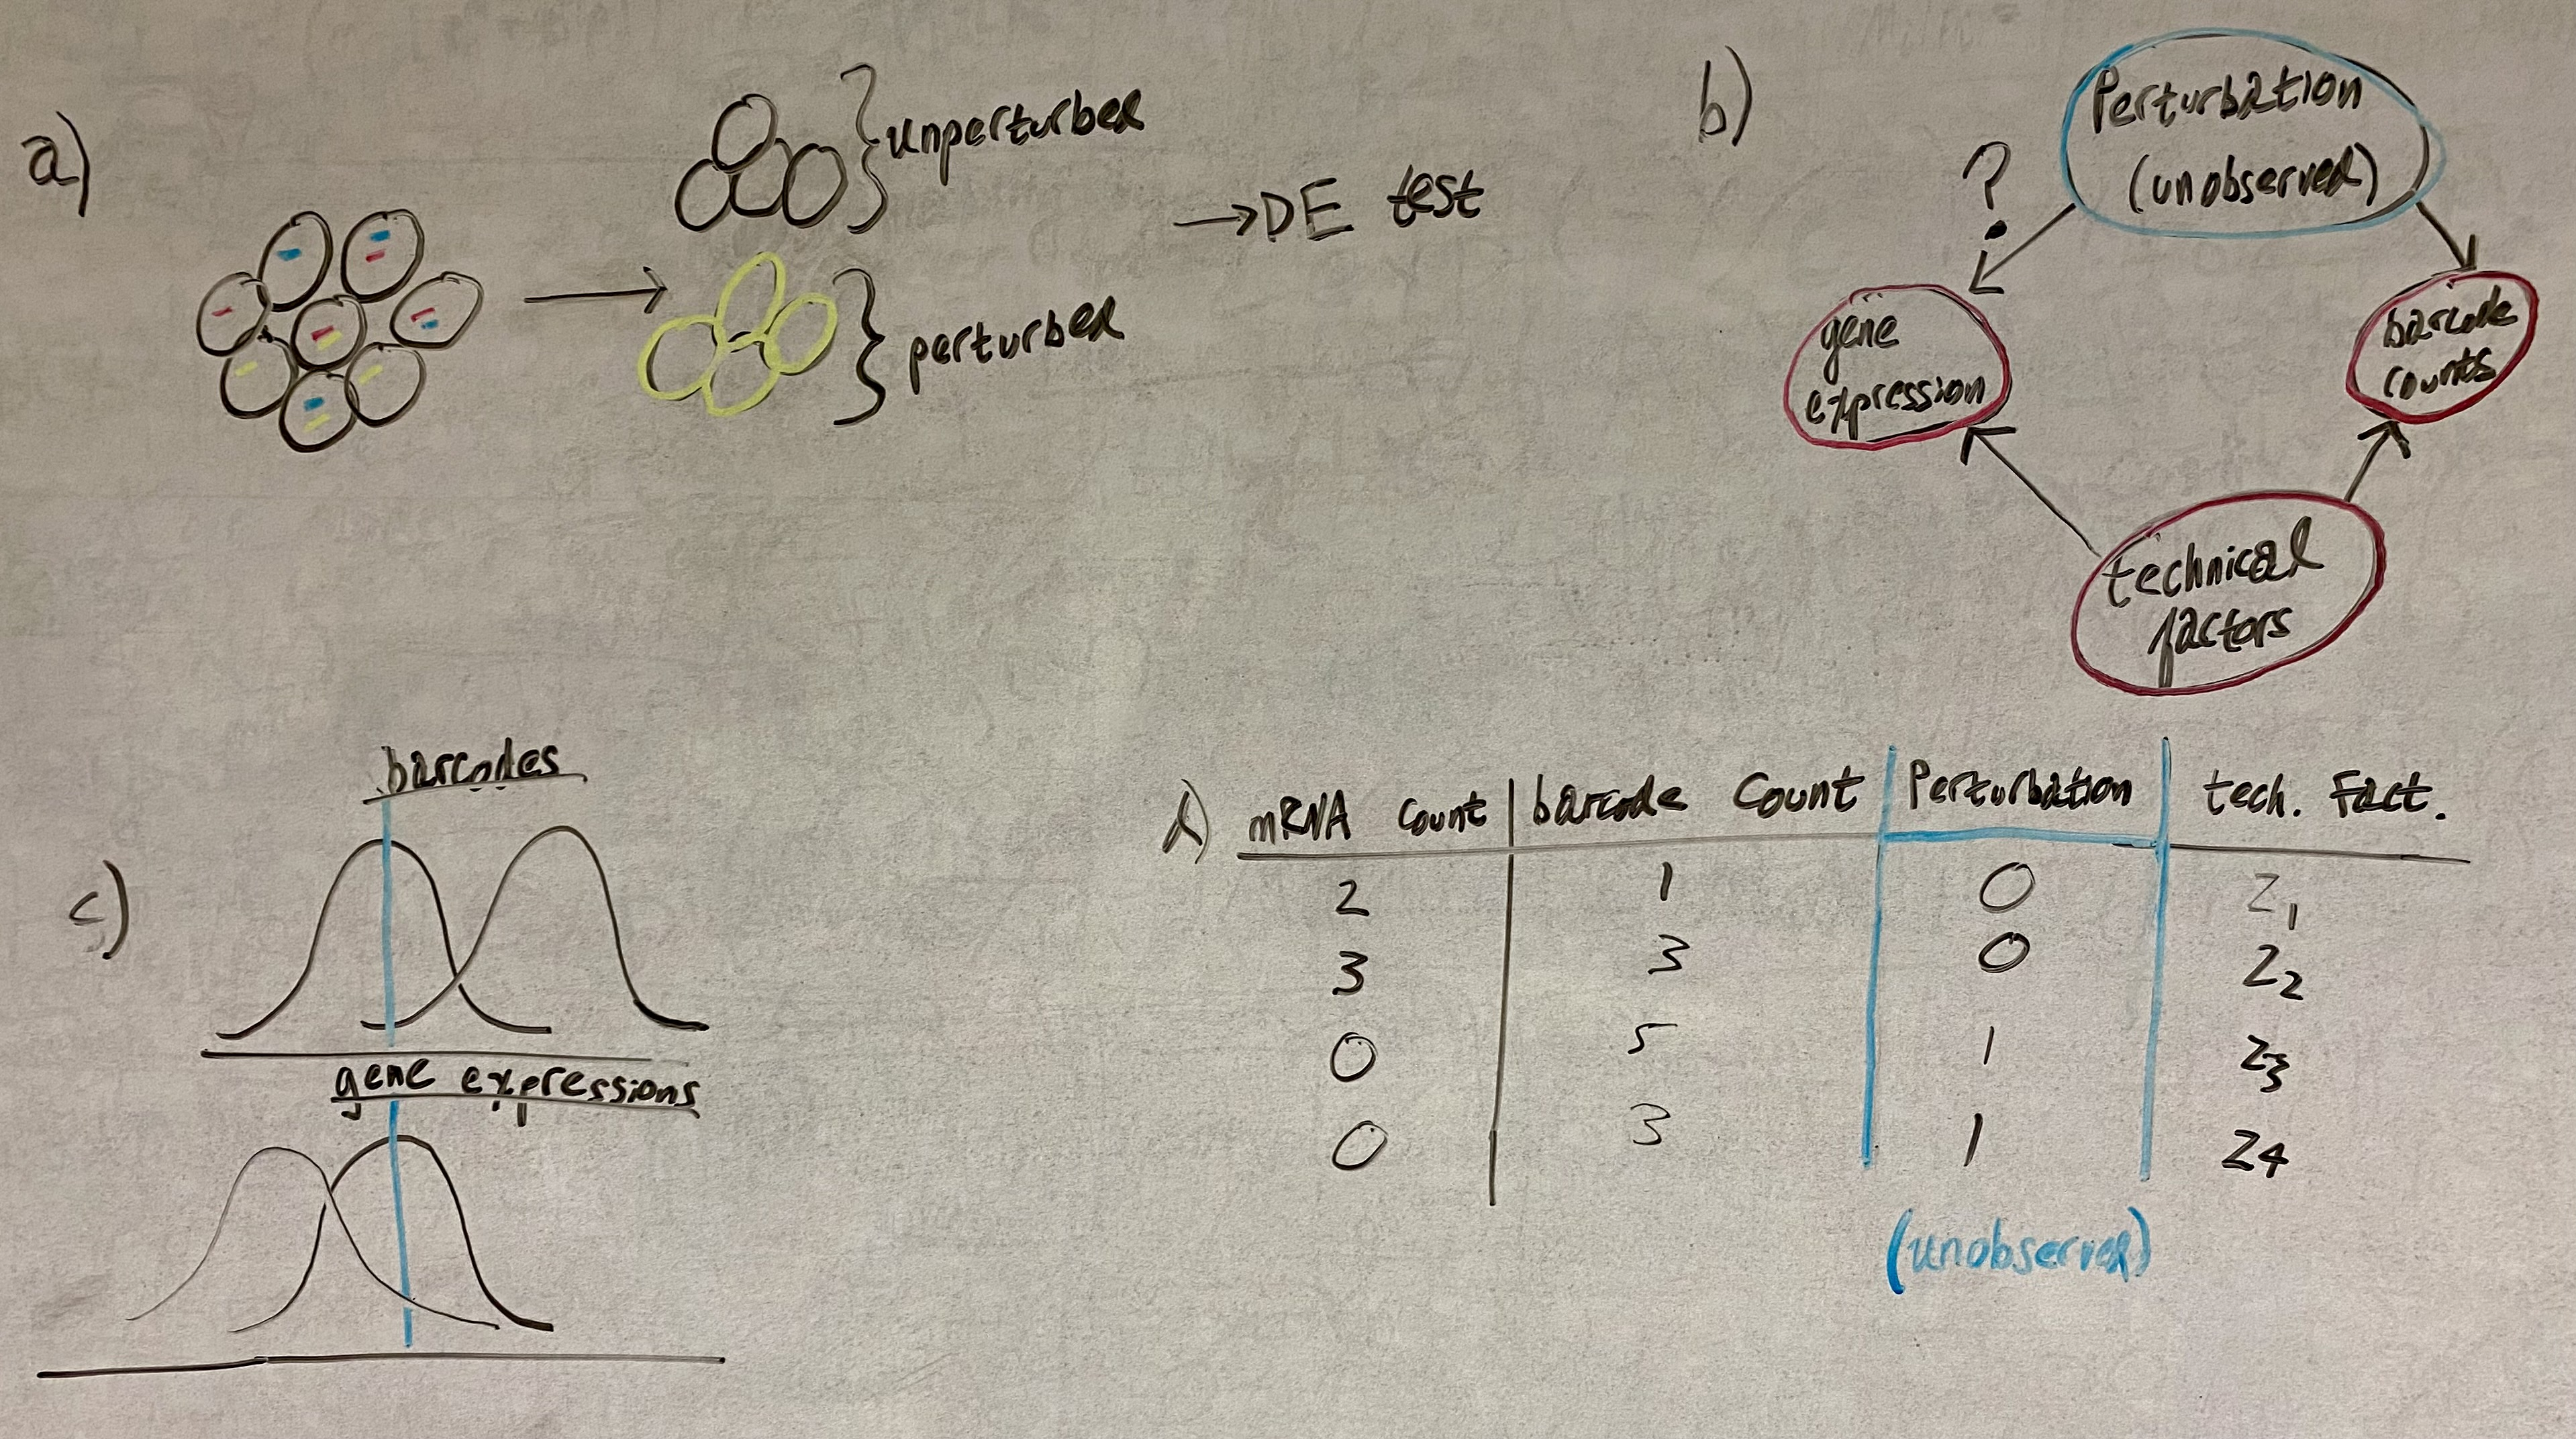
\includegraphics[width=0.9\linewidth]{analysis_challenges}
	\caption{\textbf{Overview of experimental design and analysis challenges}: \textbf{a,} Experimental design. For a given perturbation (e.g., the perturbation represented in yellow), we partition the cells into two groups: those that received the perturbation, and those that did not receive the perturbation. For a given gene, we conduct a differential expression analysis across the two groups of cells, yielding an estimate of the impact of the given perturbation on the given gene. \textbf{b,} DAG representing the variables in the analysis. The perturbation (unobserved) affects both gene expression and gRNA expression; technical factors (e.g., batch, sequencing depth, etc.) act as nuisance variables. The target of inference is the effect of the perturbation on gene expression (denoted with question mark). \textbf{c,} Schematic illustrating ``background reads.'' The gRNA modality has a nonzero, ``background read'' distribution even in the absence of a perturbation, complicating the assignment of perturbations to cells. \textbf{d}, Example data for a given perturbation-gene pair. Notice that (i) the perturbations are unobserved, and (ii) the gene and gRNA expression data take the form of discrete counts.}
	\label{analysis_challenges}
\end{figure}

\section{Related work}

Motivated (in part) by the count nature of single-cell data, several authors have generalized statistical models that (implicitly or explicitly) assume Gaussianity and homoscedasticity to a broader class of exponential family distributions. Lin et al.\ \cite{Lin2021} developed eSVD, an extension of SVD to exponential family and curved Gaussian response distributions. eSVD is better-suited than SVD to model the positive relationship between the mean and variance of a gene's expression level, which is induced by the countedness of the data \cite{Lause2021}. Along similar lines, Townes et al.\ \cite{Townes2019} proposed GLM-PCA, an extension of PCA that directly models gene expression counts while regressing out technical factors. We see our work as a continuation of this broad effort to ``port'' common statistical methods and models to single-cell count data. Our focus, however, is on regression rather than dimension reduction: we extend the classical errors-in-variables model to response distributions and sources of measurement error that are exponential family-distributed.

The closest parallels to our work the statistical methodology literature are \cite{Grun2008} \cite{Ibrahim1990}.

\section{Thresholding method}

\begin{itemize}
\item 
\item 
\end{itemize}

\subsection{Theoretical analysis}

\subsection{Empirical analysis}

\section{GLM-EIV}

\section{Simulation studies}

\section{Real data analysis}

\section{Discussion}

\section{Appendix}

% \subsection{Dictionary of symbols}

\subsection{Proofs of theoretical results for thresholding estimator}

\subsection{Derivation of EM algorithm}

\subsection{Derivation of observed information matrix}

\subsection{Implementation using R family objects}

\subsection{Statistical accelerations to GLM-EIV}

\subsection{Additional simulation results}

\bibliographystyle{unsrt}
\bibliography{/Users/timbarry/optionFiles/glmeiv.bib}


\end{document}
